\documentclass[11pt]{beamer}
\usetheme{Pittsburgh}
\usecolortheme{orchid}
\usepackage[utf8]{inputenc}
\usepackage[german]{babel}
\usepackage[T1]{fontenc}
\usepackage{amsmath}
\usepackage{amsfonts}
\usepackage{amssymb}
\usepackage{graphicx}
\usepackage{url}
\author{Patrick M\"unnich}
\title{Sigmatismus Lateralis}
%\setbeamercovered{transparent} 
%\setbeamertemplate{navigation symbols}{} 
%\logo{} 
\institute{Hochschule D\"usseldorf} 
%\date{} 
%\subject{} 
\begin{document}

\begin{frame}
\titlepage
\end{frame}

\begin{frame}
\tableofcontents
\end{frame}

\section{Der Sigmatismus Lateralis}

\begin{frame}
\frametitle{Sigmatismus Lateralis}
\begin{figure}
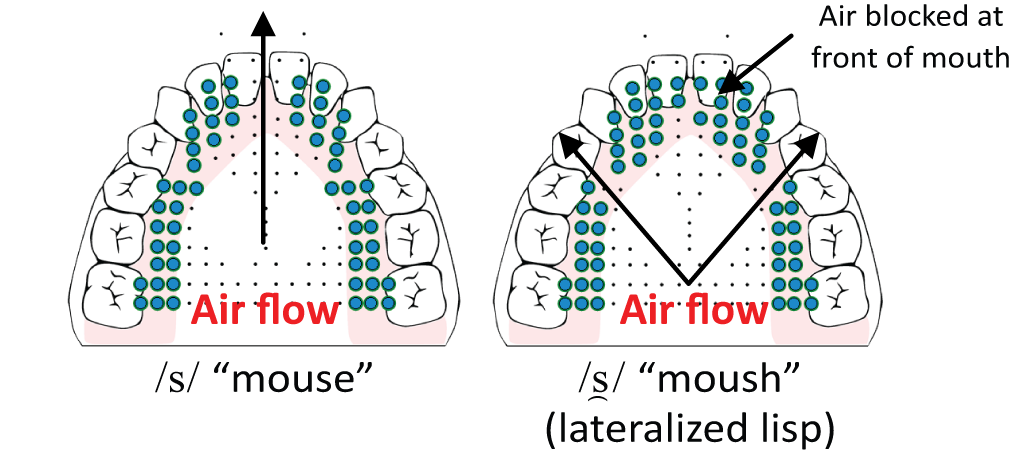
\includegraphics[scale=0.4]{lateral_lisp.png}
\caption{Sigmatismus Lateralis verglichen mit normalem S. (\url{https://www.pinterest.com/pin/7248049373293660/})}
\end{figure}
\end{frame}

\begin{frame}
\frametitle{Sigmatismus Lateralis Video}
\centering
\url{https://youtu.be/Y3mEaV1kCiU?t=21}
\end{frame}

\section{Vergleich von FFTs}

\subsection{Informationen}

\begin{frame}
\frametitle{Informationen zum Vergleich}
\begin{exampleblock}{Parameter beim Vergleich}
\begin{itemize}
\item Einfache Aufnahme mit Mikrofon neben Mund
\item 16-bit mono mit $f_\mathrm{sampling}=8000$\,Hz
\item Insgesamt drei Aufnahmen
\item Alle Aufnahmen nur ''s'' Ger"ausch mit oder ohne Lispeln
\end{itemize}
\end{exampleblock}
\begin{block}{Code}
\url{https://github.com/munnich/laterallisp}
\end{block}
\end{frame}

\subsection{Vergleich}

\begin{frame}
\frametitle{Vergleich von FFTs 1}
\begin{figure}
\includegraphics[scale=0.6]{../output/normal_vs_lisp_1.pdf}
\caption{Vergleich der FFTs vom normalen ''s'' und Sigmatismus Lateralis bei erster Aufnahme.}
\end{figure}
\end{frame}

\begin{frame}
\frametitle{Vergleich von FFTs 2}
\begin{figure}
\includegraphics[scale=0.6]{../output/normal_vs_lisp_2.pdf}
\caption{Vergleich der FFTs vom normalen ''s'' und Sigmatismus Lateralis bei zweiter Aufnahme.}
\end{figure}
\end{frame}

\begin{frame}
\frametitle{Vergleich von FFTs 3}
\begin{figure}
\includegraphics[scale=0.6]{../output/normal_vs_lisp_2.pdf}
\caption{Vergleich der FFTs vom normalen ''s'' und Sigmatismus Lateralis beidritter Aufnahme.}
\end{figure}
\end{frame}

\subsection{Festellungen}

\begin{frame}
\frametitle{Feststellungen bei Vergleich von FFTs}
\begin{itemize}
\item[$\Rightarrow$] Bei allen drei Aufnahmen offensichtlich viel mehr im h"oheren Frequenzbereich (ca.\ 1200-3500\,Hz)
\item[$\Rightarrow$] Ansatz: man sollte durch Vergleich der h"oheren Frequenzen zwischen normalen ''s'' und Sigmatismus Lateralis unterscheiden k"onnen
\end{itemize}
\end{frame}

\section{Formanten}

\begin{frame}
\frametitle{Betrachtung der Formanten mit Praat}
Screenshots w"aren hier leider zu gro"s
\begin{block}{Ergebnisse}
\begin{enumerate}
\item Formant normal zwischen 700-800, Lispeln 500-700
\item Formant normal zwischen 1500-2000, Lispeln 1800-2200
\item[$\Rightarrow$] Schien konsistent "uber alle Aufnahmen
\end{enumerate}
\end{block}
\end{frame}

\end{document}